\section{Implementation}
\subsection{GUI and IDE}
\label{IDE}
\subsubsection{Introduction}

The GUI and IDE are both implemented in JAVA with the JHotDraw 7.1 framework. 
Early on it was decided that the GUI functions like other popular tools for 
drawing flow charts such as Visio, IBM's Rational software, and Dia. 
All of these tools are interactive in the drawing of the diagram rather than 
compile a graph from a descriptive language. The reason for enforcing interactive 
drawing is that this tool is designed to simplify the original implementation 
of ladder logic, and building it on a textual graphical language will
significantly hurt the primary goal of ease of use.
JAVA was chosen for portability as it was simpler to deploy a JAVA implementation 
than multiple ports for each target in the the short duration of this project.

The GUI itself remains minimal there is a toolbar in which objects can be 
selected from the tools palette and drawn. Properties of an object are 
directly editable on the object itself once drawn instead of a separate 
property palette. Again this design decision was chosen as it is more 
immediately understandable and intuitive to the user, rather than for 
power and expressiveness.

%figure goes here
\subsubsection{Using The GUI: Parts of the GUI}

\subparagraph{The Main Canvas}

\begin{figure}[htp]
    \centering
    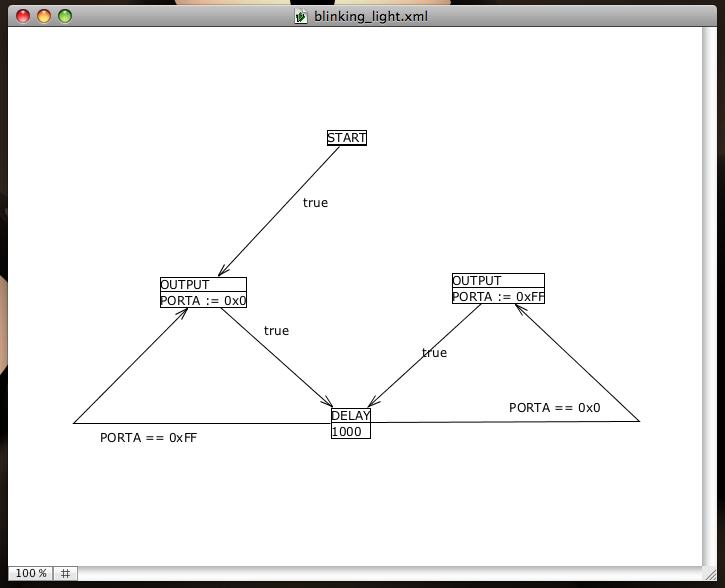
\includegraphics[width=\imgmedium]{./images/plcedit_canvas.png}
    \caption{The Drawing Canvas}
    \label{fig:plcedit_canvas}
\end{figure}

The main canvas represents the main working area for the user as shown 
in Figure \ref{fig:plcedit_canvas}. As one would expect from a drawing
program the canvas can be scrolled by using the horizontal and vertical 
scroll bars. In addition the drawing can also be zoomed in and out by 
using the zoom buttons located at the bottom of the canvas. Object 
manipulation is accomplished by selecting the appropriate tool from the 
tools palette then manipulate the object directly in the drawing canvas.

\subparagraph{The Tools Palette}

\begin{figure}[htp]
    \centering
    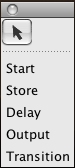
\includegraphics[width=50px]{./images/plcedit_tools.png}
    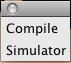
\includegraphics[width=50px]{./images/plcedit_actions.png}
    \caption{The Tools Pallette}
    \label{fig:plcedit_tools}
\end{figure}

The tools palette is were the user selects their tool to use on the 
canvas shown in Figure \ref{fig:plcedit_tools}. Only one tool can be 
used at a time. All tools except for compile and simulation are selected
for use on click. Compile and simulation are immediately executed on click.
The tools listed on the tools palette are as shown in Figure  \ref{fig:plcedit_tools}
and have the functionality as follows.

\begin{itemize}
\item \textbf{Selection Tool}: This tool allows you to select one or multiple objects. Or edit properties of objects. You can move the object around the canvas by first selecting the object with a single click, then clicking and dragging the object to the desired location. Editing properties are accomplished by double clicking the property you would like to edit on the object itself.

\item \textbf{Transition Tool}: This tool draws transitions between one block to another. Before you draw a transition you must have created the two blocks you wish to connect. To draw the transition you start by clicking and holding down the left mouse button over the starting block then dragging until the line snaps over the ending block. On release of the left mouse button a transition is formed and the two blocks are linked. For layout purposes you may also double click on a transition  line to add more anchors.

\item \textbf{The Start Tool}: The code will give a compile error if more than one start block is placed on the diagram. Start blocks have no other data associated with them but they serve as the starting point of your program when the PLC unit is first turned on. Your diagram must contain exactly one start block and there must only be one edge leaving the start block. No variables or guard conditions can be evaluated at the start of the program since the controller is still uninitialized so the result of the guard conditions is entirely dependent on what the chip has at these memory locations.

\item \textbf{The StoreBlock Tool}: You can use these blocks to perform calculations or update internal variables. To begin drawing a store block you first select this tool. Then you click on the canvas where you would like it to appear. Store blocks are auto-resizing objects thus the size is determined by the content. To edit each field in a store block you double click the parameter you wish to edit. If you wish to delete a line you can simply erase the identifier. If you wish to add a new line change the last identifier to something other than the default placeholder value. A new placeholder will be created as soon as you perform this action in order to allow you to add more lines.

\item \textbf{The Delay Tool}: Delay blocks are used to insert a specified delay into your program the length of the delay is specified in milliseconds. When an edge is taken to the delay block the code execution is delayed and none of the departing edges are taken until the delay time specified has elapsed. It is often useful to have your program wait for a specified period, although the same can be achieved by using a store block and a counter update it is far easier and more accurate to use the dedicated delay block.

\item \textbf{The Output Tool}: Output blocks are used to send outputs from the program to pins on the PLC itself. Depending on the chip type there can be one or many different output ports. Each port is a 8-bit representation of the pins, an expression is also allowed on the right hand side so masking could be done.

\item \textbf{The Input Tool}: Similar to the format of the output block the input block allows you to read data from one or many ports (depending on hardware) into an internally used variable.

\item \textbf{Compile Action}: Executing the compile action will start the compilation process into PLC \emphasize{IL} (intermediate Language) code this code is directly compilable on targets that have implemented the hardware framework which is discussed in detail in Section \ref{sec:hardwareframework}.

\item \textbf{Simulator Tool}: The simulator action brings up a tracing and debugging window. This window allows you to step through each of the code blocks to simulate what might happen as your program runs.
\end{itemize}

\subparagraph{Compile Preview Window}

\begin{figure}[htp]
    \centering
    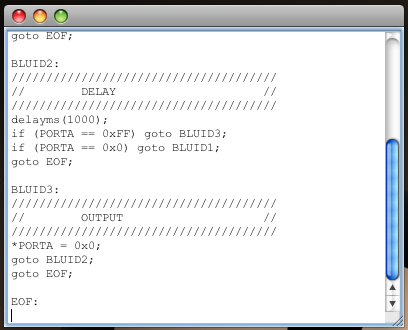
\includegraphics[width=\imgmedium]{./images/plcedit_compile.png}
    \caption{Compile Preview Window}
    \label{fig:plcedit_compile}
\end{figure}

After the compile button is invoked the compile preview window is presented as shown in Figure \ref{fig:plcedit_compile}. The preview window serves as a quick overview of the program code that can be loaded onto the device. The user then has the option of saving the text off to a compilable file for loading onto the device.

\subparagraph{Simulator Window}

In order to aid in debugging a simulator mode has been added to the visual editor. When the simulator window is brought up it helps the programmer visually identify what their current memory layout looks like as well as which block they are currently executing. In Figure \ref{fig:plcedit_simulator_start} the following view is presented right after the simulator button has been invoked. Note the contents of all variables and all ports are shown. Also the start block is automatically highlighted and the ports are initialized to their starting values.

The \emphasize{Step Once} button allows the user to to step through the current block one step at a time. The \emphasize{Step Next} button finishes all operations in the current block and jumps directly to the next block. Figure \ref{fig:plcedit_simulator_running} demonstrates what the program might look like after a it is allowed to run for a few steps.

\begin{figure}[htp]
    \centering
    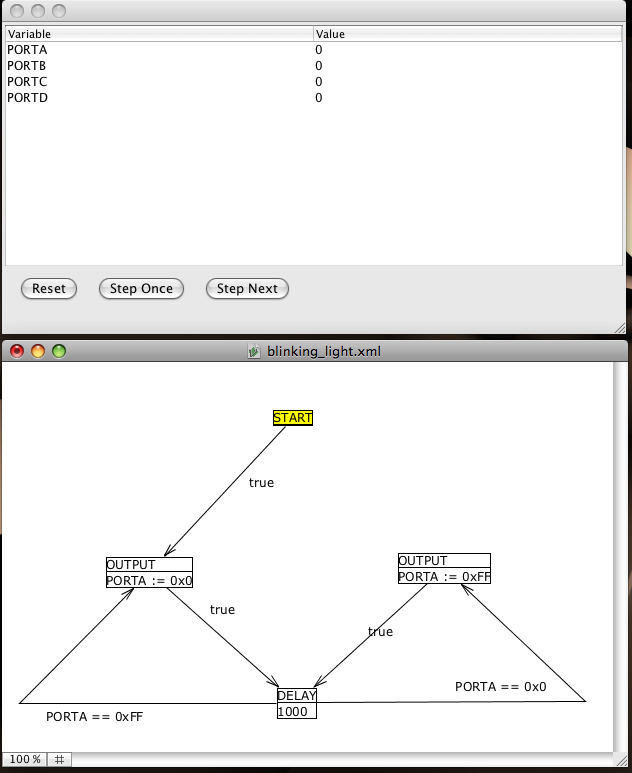
\includegraphics[width=\imgmedium]{./images/plcedit_simulator_start.png}
    \caption{Simulator Window Starting Configuration}
    \label{fig:plcedit_simulator_start}
\end{figure}



\begin{figure}[htp]
    \centering
    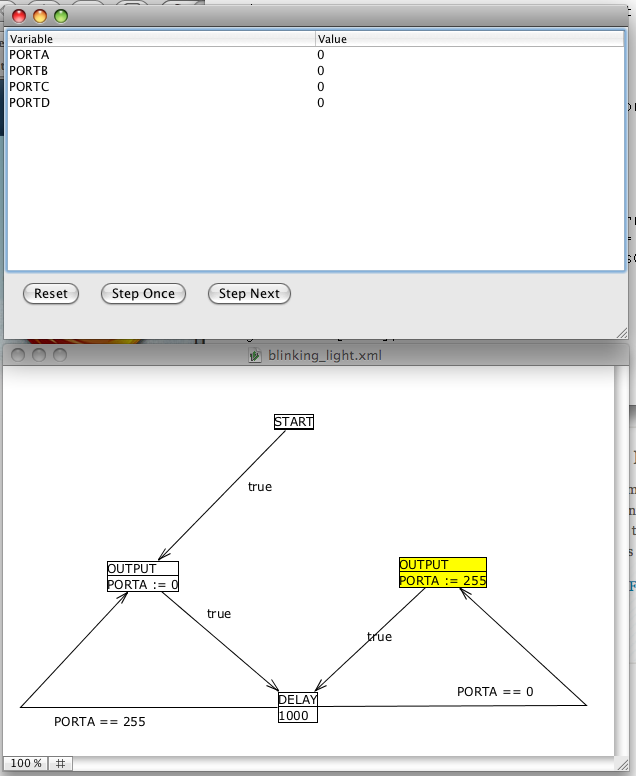
\includegraphics[width=\imgmedium]{./images/plcedit_simulator_running.png}
    \caption{Simulator Window Program Running}
    \label{fig:plcedit_simulator_running}
\end{figure}





\subsection{Data Flow}

Construction of the final compiled code starts at the GUI level. The designer starts 
by drawing the layout of the program they wish to construct. This drawing forms 
the basis of the underlying code structure. The designer then tests the behaviour of 
their program by utilizing the simulation tools. Once satisfied the designer uses the 
compile tool to generate the final program code. This program code is then compiled onto 
the final architecture by the embedded hardware compilation tools. Any hardware that 
has implemented the support required by the hardware framework (which is discussed in 
detail in Section \ref{sec:hardwareframework}) will run compile and run this program code.

\subsection{Generated Code Structure}
\label{sec:implementation:struct}
The structure of each compiled section was carefully constructed to preserve the 
structure of the drawn graph as closely as possible. The basic structure of 
each compiled block can be seen as follows:

\begin{definition}
\label{def:genCodeStruct}
Structure of \plcchart \  generated code

\begin{lstlisting}[frame=single]
BLUID5:
//////////////////////////////////
//// Block Header               //
//////////////////////////////////
(Program Code)

if ( guard condition ) goto BLUID2;
goto EOF;
\end{lstlisting}
\end{definition}

As you can observe from Definition \ref{def:genCodeStruct} each code block
generation first starts with a \emphasize{BLUID} (Block Unique Identifier).
The purpose of the \emphasize{BLUID}'s is to give a reference point for the
start of the block having a \emphasize{BLUID} label for each block enables
any block to be jumped to should we want to. The block header which comes 
right after is an identifier to the type of block being generated. 

In the ``(Program Code)'' section of Definition \ref{def:genCodeStruct} 
sits the generated \emphasize{IL} code. This code is the same for each target platform. 
Each \emphasize{IL} target will have appropriate implementations that will map \emphasize{IL} 
calls to hardware specific calls. These calls can be found in Section \ref{sec:hardwareframework}. 
The generated \emphasize{IL} code resembles C code with specific calls to lower level 
functions that are supported by the PLC target's hardware framework.

The final block of if statements implement the edges leaving the block. 
Each edge is guarded by an if statement, and will have the goto portion 
point the the correct \emphasize{BLUID} as specified by the diagram. 
\emphasize{goto} was chosen over conventional control structures as it
provided several advantages. The first is that translation from graph 
structure to code is fundamentally easier. \emphasize{goto}'s are analogous 
to graph edges where trying to analyze the diagram and fit structures 
like \emphasize{for} \emphasize{while} are inherently much harder and 
prone to error. In addition these structures are more at home in textual 
programming languages and do not improve the structure of the 
graphical programming language. The next advantage was during code 
generation when trying to unroll structure from our graphical programming language 
not using \emphasize{goto}'s will cause the order of items to be important. This
makes it necessary to form a dependency tree of blocks to each other if they 
started requiring each other. All these problems were easily avoided by staying 
with a simple goto structure inside the actual 
generated \emphasize{Intermediate Language} code itself. The trade off in this 
design decision is the resulting generated code becomes a machine 
generated code and is not very user editable. 

Finally if at any point no edges are valid the the program will 
terminate by going to the label ``EOF'' which will be located 
at the end of the file.


\subsection{Compiled Structure}
\label{compiler}

Each of the blocks will compile their own snippets of code. 
It may be helpful when reading this section to refer to 
Definition \ref{def:genCodeStruct} for the generic block 
structure definition. Each block primative's construction
is detailed below.

\subsubsection{Start Block}
\label{def:cmpstartblock}
\begin{lstlisting}[frame=single]
00 BLUID#:
01 //////////////////////////////////////
02 //        PROGRAM START             //
03 //////////////////////////////////////
04 
05 if (condition) goto LABEL;
06 goto EOF;
\end{lstlisting}

The primary function of a start block is to provide a block that 
can have edges directed at it, and to give a starting point for 
the program. Line 00 is the ``block unique identifier'' as stated 
in Definition \ref{def:genCodeStruct} this is used by other blocks 
when edges are directed at this block. Lines 01-03 is a block 
description without this it becomes difficult to 
determine what kind of block is executing if the code needs to 
be examined by human eyes. 

On line 06 the standard ``goto EOF'' is generated to ensure if no 
edges exist the program will stay in the block and not execute any 
other block by going to the end of the program.

\subsubsection{Delay Block}
\label{def:cmpdelayblock}
\begin{lstlisting}[frame=single]
00 BLUID#:
01 //////////////////////////////////////
02 //        DELAY                     //
03 //////////////////////////////////////
04
05 delay_ms(integer);
06 
07 if (condition) goto LABEL;
...
08 goto EOF;
\end{lstlisting}

Since the structural components are identical to the code sample 
provided in the ``Start Block'' we will skip lines 00-04. Unlike 
the ``Start Block'' the ``Delay Block'' does perform an operation 
during execution. On line 05 the ``Delay Block'' calls 
delay\_ms(\textbf{integer}) where \textbf{integer} refers to the 
integer specified in the diagram. The routine for delay is done 
on the hardware side as the manufacturer will choose how to appropriately
determine 1ms on hardware. \texttt{delay\_ms} is a call that will
be implemented on the hardware framework show in Section \ref{sec:hardwareframework}.

\subsubsection{Input Block}
\label{def:cmpinputblock}
\begin{lstlisting}[frame=single]
00 BLUID#:
01 //////////////////////////////////////
02 //        INPUT                     //
03 //////////////////////////////////////
04
05 variable = PORTIN;
06 
07 if (condition) goto LABEL;
     ...
08 goto EOF;
\end{lstlisting}

The input routine performs an operation of setting a variable 
to the value being read off the input port. This value is located 
on line 05 ``variable = PORTIN;''. Lines 00-04 are the same as 
Definition \ref{def:genCodeStruct} and line 07-08 are identical 
to the Delay block. In this case variable can be any variable in
our program that can accept a 8 bit integer values.


\subsubsection{Output Block}
\label{def:cmpoutputblock}
\begin{lstlisting}[frame=single]
00 BLUID#:
01 //////////////////////////////////////
02 //        OUTPUT                    //
03 //////////////////////////////////////
04
05 PORTOUT = variable;
06 
07 if (condition) goto LABEL;
     ...
08 goto EOF;
\end{lstlisting}

The ``Output Block'' is nearly identical to the ``Input Block'' 
the only difference is on line 05 instead of reading a value from 
the input port a value is written to the output port. This is 
accomplished by the line ``PORTOUT = variable;''.

\subsubsection{Store Block}
\label{def:cmpstoreblock}
\begin{lstlisting}[frame=single]
00 BLUID#:
01 //////////////////////////////////////
02 //        STORE                     //
03 //////////////////////////////////////
04
05 variable0 = expression0;
06 variable1 = expression1;
07 variable2 = expression2;
     ...
08 if (condition) goto LABEL;
     ...
09 goto EOF;
\end{lstlisting}

Again we start the store block similar to the other blocks with 
identical structure until line 04. Line 05-07 are the code conversions 
for the store block. The store block converts each line in the diagram 
of the form ``type variable\_name := expression'' into ``variable\_name = expression'' 
as seen on line 05. In addition if there is more than one line they 
are then placed one after the other in sequence. The expressions used can be any 
valid mathematical ``C'' style expression. Functions calls used in the 
expressions are not supported.